\section{Semantics theory}\label{sec:semantic}
\emph{''Programming language semantics is the study of mathematical models of and methods for describing and reasoning about the behaviour of programs.''}\cite{transtrees}\\
The before citation pretty much sums up the whole meaning of semantics, in detail it means that programming language semantics describe the inner workings of a program in a mathematical form.\\
Two forms of operational semantics are generally used when describing program behaviour, ''Big-step'' and ''Small-step''.
Big-step semantics describe an entire computation in a single transition;
$ \gamma \rightarrow \gamma' $.
Where $\gamma'$ is always a terminal configuration.
small-step semantics describe a single step of a larger computation in a transition and the $ \gamma' $ is not necessarily a terminal configuration.\\
Both have their pros and cons, Big-step semantics are easier to formulate than the other, sacrificing details in the process and not able to describe non-terminating programs. Small-step semantics can be quite complex to formulate and in contrast to big-step, have detail and describe all types of programs terminating or non-terminating.\cite{opsemantics}\cite{transtrees}

\subsection{Environment-store model}\label{subsec:env-sto}
The semantics of \langname{} are described with the help of the environment-store model. Environment-store describes how variables are bound during a program execution. Each variable is bound to a storage cell, and the content of the storage cell is the value of the variable.

The below example is exactly as the one presented in Transitions and Trees \cite{transtrees}. It is a visual representation of the environment-store model and how it works. The difference between this one and the also used \emph{''state''- model} is that the environment-store model provides more details regarding as where changes take place during execution.
\begin{figure}[!h]
\centering
	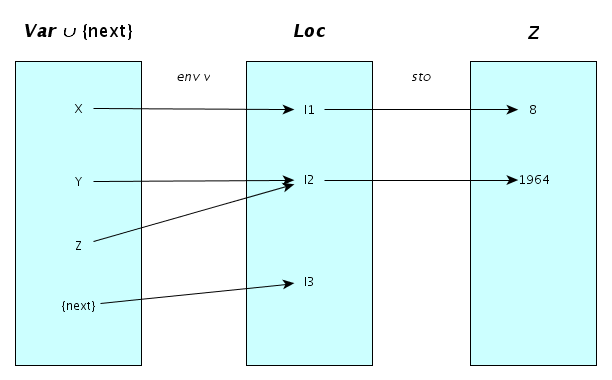
\includegraphics[scale=0.55]{img/envstore.png}
	\caption{Example of a variable environment and a store \cite{transtrees}}
\end{figure}\\
As can be seen, there are three variables plus a reference called \texttt{\{next\}}, which always points to the next available location. What can not been seen is the function \texttt{new}, which always points to the new location, whether the location is available or not. 
\begin{description}
\item Variable $X$ is bound to location $l_1$, which points to a store containing the integer '8'.
\item Variable $Y$ is bound to location $l_2$. which points to a store containing the integer '1964'.
\item Variable $Z$ is bound to location $l_2$ like $Y$ is, the location points to the same integer as before.
\item Reference \texttt{\{next\}} is bound to location $l_3$, as it is not bound to any variable and therefore is unassigned.
\end{description}
%\\\\
In mathematical form, both environment and store are presented. As mentioned before this model provides more details and is due to the fact that when data changes (e.g assignments) the store is presented with a ' symbol and when a new class is created within a specific environment the environment is presented with a ' symbol. Opposed to 'state'- model where the state is presented with a ' symbol to indicate all changes.